\documentclass{article}

\usepackage{graphicx}
\usepackage{lmodern}
\usepackage{enumitem}

\begin{document}
	\begin{titlepage}
		\fontfamily{pbk}\selectfont
		\hbox{			
			\rule{1pt}{\textheight}
			\hspace*{0.05\textwidth}
			\parbox[b]{\textwidth}{
				\Large Project Tender\\[1cm]
					
				\Huge Project: Harvest\\
				\huge Client: Subtrop\\[1.5cm]					
					
				{\huge Team: HTTP\textunderscore418}
				
				\begin{itemize}[label={}, leftmargin=0pt, noitemsep]
					\Large						
					\item Christiaan Saaiman, 12059138
					\item Michael Loosen, 14017254
					\item Elizabeth Bode, 14310156
					\item LC Meyers, 14024633
				\end{itemize}
				\vspace{0.5cm}
					
				{\large Department of Computer Science, University of Pretoria\\[0.2cm]}

				\Large\today\\[0.3cm]				
									
				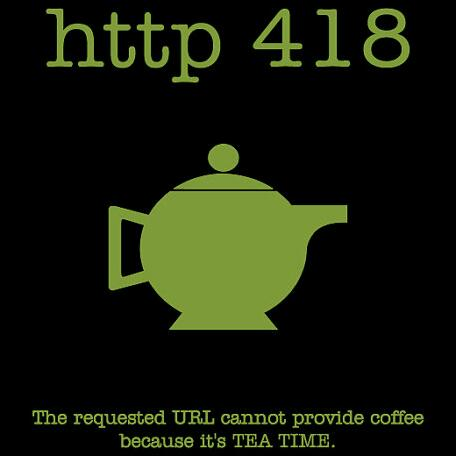
\includegraphics[scale=0.3]{../teamPic.jpg}					
			}								
		}
	\end{titlepage}
	\newpage
	\section{The Team}
	\subsection{LC Meyers}
	\begin{figure}[h]
		\centering
		
\includegraphics[height=0.3\textheight]{../charl.jpg}
	\end{figure}
	\begin{itemize}
		\item \textbf{Full name:} Lodewyk Charles Meyers
		\item \textbf{My interests:}
			\subitem Gaming
			\subitem Computers
			\subitem Music
			\subitem User experience design
			\subitem Website design
			\subitem Anything new related to technology
		\item \textbf{My technical skills:}
			\subitem Web development skills
			\subitem Database design
			\subitem Java
			\subitem C\#
		\item \textbf{Past experience that might help:}
			\subitem I have collaborated in an Android app made using PhoneGap
		\item \textbf{Non-technical strenghts:}
			\subitem I have a high amount of patience
			\subitem Hardworking
			\subitem Eager to learn new things
			\subitem Enjoy trying to solve complex problems
		\item \textbf{What makes me want to do this project?} Doing  this project sounds like it can be fun. It sounds like I might learn something new in the Subtropical industry. It will also be interesting to see how the service is being realised to help the farmers determine better yields. Finally it would be nice to learn how to create an app that uses GPS and other technologies needed for this project.
	\end{itemize}
	
	\section{Project excecution}
	\paragraph{Details go here}
\end{document}